\documentclass[12pt]{article}
\usepackage{graphicx}
\usepackage{eso-pic}
\usepackage{ragged2e}
\renewcommand\thepage{- \arabic{page} -}
%Logo
\newcommand\Highlight{%
	\put(0,150){%
		\parbox[b][\paperheight]{\paperwidth}{%
		\vfill
		\centering
		
\includegraphics[width=\paperwidth, height=10cm]{logo.jpg}%
		\vfill
}}}
%Swirl
\newcommand\Swirl{%
	\put(50,270){%
		\parbox[b][\paperheight]{\paperwidth}{%
		\vfill
		\centering
		
\includegraphics[width=20cm, height=20cm]{background.png}%
		\vfill
}}}
\usepackage{graphicx}
\graphicspath{{../images/}}

\AddToShipoutPicture*{\Highlight}
\AddToShipoutPictureBG{%
	\ifnum\value{page}>1
	\AtPageLowerLeft{\Swirl}%
    \fi
    }%

\begin{document}

{\fontfamily{phv}\selectfont % change phv to get new fonts for whole document
\font\myfont=cmr12 at 20pt

\begin{center}


\begin{minipage}{0.75\linewidth}


\vspace*{250pt}
\title{ \rule{\linewidth}{2pt} \\
\textbf{\normalfont\fontsize{35}{35}\scshape\selectfont IoT HomeCare System}\\
\textbf{\normalfont\fontsize{35}{35}\scshape\selectfont Testing}\\}
\author{
        Hristian Vitrychenko\\
        Nikki Constancon \\
        Juan du Preez\\
        Gregory Austin \\
        Marthinus Richter
}
\date{\today \\ \rule{\linewidth}{2pt}}


\maketitle
\thispagestyle{empty}

\end{minipage}
\end{center}
\pagebreak
	\section{Introduction}

	The testing report is designed to describe all tests that have been done on the system and future tests to be done on the system.

		\subsection{Purpose}

		The purpose of this document will be to list and describe all of the tests for the ReVA system, how they are carried out, what their purpose is and what subsystem and related module(s) they are related to.

		\subsection{Structure of the document}

		Each subsystem of ReVA will be addressed individually with the specific tests for each module concerned with that subsystem. The subsystems are:
		\begin{itemize}
			\item Real-Time Subsystem \\ This includes the modules: Data Collection,  Pub/Sub Server, Data Pull, and User Interface
			\item Data Storage Subsystem \\ This includes the modules: Data Storage, Pub/Sub Server
			\item History/Statistics Subsystem \\ This includes the modules: Data Storage, Statistics, Pub/Sub Server, and User Interface
			\item User Management Subsystem \\ This includes the modules: User Management, User Interface
			\item Notification Subsystem \\ This includes the modules: Pub/Sub Server, Notification, and User Interface
			\item Advice Subsystem \\ This includes the modules: Advice and User Interface
		\end{itemize}
		\subsection{Definitions, Acronyms, and Abbreviations}


			\subsubsection{Acronyms}

			\begin{itemize}

				\item \textbf{UI} \textbf{\textit{(User Interface)}} \\
				\newline
				The means by which the user and a computer system interact, in particular, the use of input devices and software.

			\end{itemize}

			\subsubsection{Definitions}

			\begin{itemize}

				\item \textbf{Unit Test}\\
				\newline
				Unit testing is a software development process in which the smallest testable parts of an application, called units, are individually and independently scrutinised for proper operation.\\
				\item \textbf{Integration Test}\\
				\newline 
				Find out if the units if integrated together will work without errors. For example, argument passing and data updation etc.
				\item \textbf{Functionality Test}\\
				\newline 
				Tests all functionalities of the software against the requirement.
				\item \textbf{Performance Test}\\
				\newline 
				This test proves how efficient the software is. It tests the effectiveness and average time taken by the software to do desired task. Performance testing is done by means of load testing and stress testing where the software is put under high user and data load under various environment conditions.
				\item \textbf{Alpha Testing}\\
				\newline 
				The team of developer themselves perform alpha testing by using the system as if it is being used in work environment. They try to find out how user would react to some action in software and how the system should respond to inputs.

			\end{itemize}

		\subsection{Additional Information}

		The code being tested is written by different developers, thus this document serves as a way in order to review the functionality and tests done, and to provide information about future tests on future or current functionality.\\\\


	\pagebreak

	\section{Real-time subsystem}
	\textbf{Modules involved:} Data Collection,  Pub/Sub Server, Data Pull, and User Interface \\
	\textbf{Implementation status:} implemented \\
	\textbf{Primary Actors:} All users \\
	\textbf{Functionality:} View real time data on patient(s)\\
	\subsubsection{Description of current tests}
	The data streaming consists of Raspberry pi's streaming to servers, and servers streaming that data out and the application displaying those data streams. We do this using the Nodejs package Zetta (which is already been tested) for the Data Collection and the Pub/Sub Server, and an open source Zetta-Starter-Android-Application developed to interface with the Zetta API to recieve the streams (DataPull) that's generated by the server which has also been tested. These have all been tested individually already, thus to create our own unit tests would be redundant.
	\subsubsection{Future tests:}
	Future tests will include Integration Testing, Functionality Testing to confirm it adheres to requirements, Performance testing (seeing capacity and application performance) and some Alpha Testing (testing it ourselves to potentially find problems).
	\subsubsection{Data Collection}
	\textbf{Comment:} At the moment the Pi collects data from mock devices. This data generated and streamed using the zetta architecture and therefore has already been tested with Unit tests thoroughly. (Zetta is an open source Nodejs project purposed for IoT)
	\subsubsection{Pub/Sub Server}
	\textbf{Comment:} The Pub/Sub server uses zetta architecture as well and that's how it communicates with the pi (recieves streams being published) and any requesting devices looking to subscribe. Zetta already is established and has tests.
	\subsubsection{Data Pull}
	\textbf{Comment:} The way the data is pulled is by using the architecture of the open source Zetta-Starter-Android-Application developed to interface with the Zetta API that's generated by the server. This has also been tested, so testing is redundant.
	\subsubsection{User Interface}
	\textbf{Comment:} The user interface only displays data, and therefore it is easy to verify what is being displayed and that it is working as expected.
	
	
	\begin{figure}[h!]
		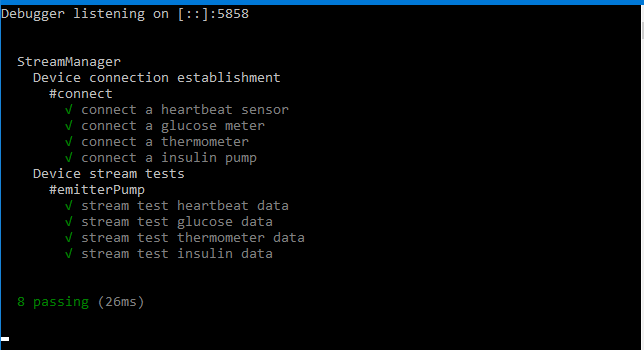
\includegraphics[width=\textwidth]{tests/zettaStream/test-zetta-stream-pass}
		\caption{Mocha output of successful mock device streams}
	\end{figure}
	\begin{figure}[h!]
		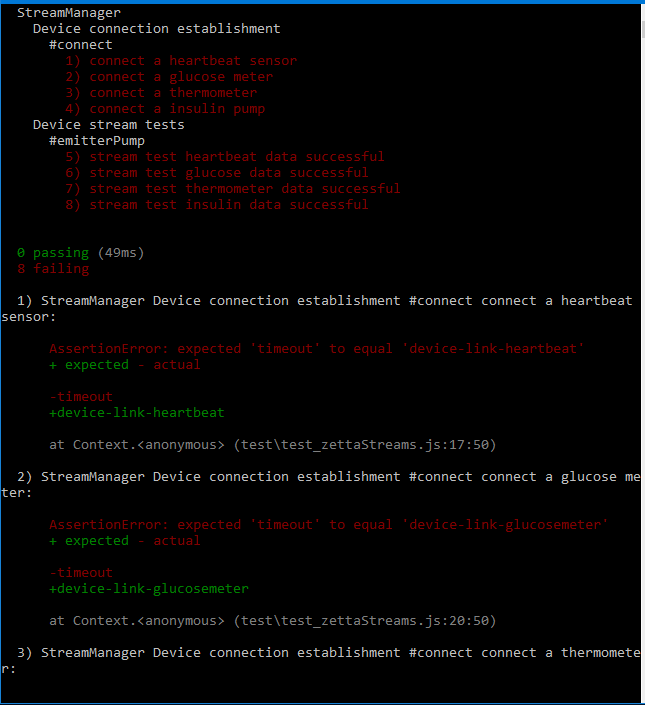
\includegraphics[width=\textwidth]{tests/zettaStream/test-zetta-stream-fail00}
		\caption{Mocha output (1 of 2) for unsuccessful mock device streams (due to being programmatic disabled)}
	\end{figure}
	\begin{figure}[h!]
	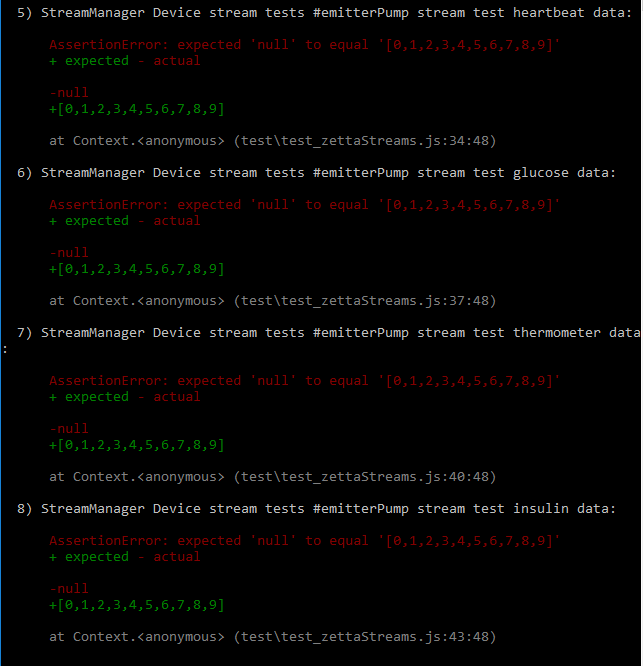
\includegraphics[width=\textwidth]{tests/zettaStream/test-zetta-stream-fail01}
	\caption{Mocha output (2 of 2) for unsuccessful mock device streams (due to being programmatic disabled)}
	\end{figure}
	
	
	%!!!!!!!!!!!!!!!!!!!!!!!!!!!!!!!!!!!!!!!!!!!!!!!!BREAK!!!!!!!!!!!!!!!!!!!!!!!!!!!!!!!!!!!!!!!!!!!!!!!
	\pagebreak
	%!!!!!!!!!!!!!!!!!!!!!!!!!!!!!!!!!!!!!!!!!!!!!!!!BREAK!!!!!!!!!!!!!!!!!!!!!!!!!!!!!!!!!!!!!!!!!!!!!!!

	\section{Data Storage Subsystem}
	\textbf{Modules involved: } Data Storage, Pub/Sub Server \\
	\textbf{Implementation status:} unimplemented \\
	\subsubsection{Future tests:} Unit tests for individual modules, Data Storage in particular because the Pub/Sub server is zetta. There will also be Integration Testing to make sure that data storage and the pub/sub server are passing messages as expected. 

	\section{History/Statistics subsystem}
	\textbf{Modules involved:} Data Storage, Statistics, Pub/Sub Server, and User Interface
	\textbf{Implementation status:} unimplemented
	\subsubsection{Future tests:} Unit tests for data-storage, statistics and the user interface. For data-storage this will include unit tests to verify statistical/historical data is stored and timestamped correctly. For statistics this will include unit testing for verification of getting the right data from queries, as well as any mathematics done by the statistics module, e.g., min, max, avg, mean etc. The user-interface will need unit-testing to make sure that graphs are being shown as specified, or statistics about the patient are indeed correct. Other tests will include integration testing in the future to make sure everything is communicating as expected. There will also be functionality testing to be sure that the History/Statistics subsystem meets the SRS accurately. 

	\section{User Management Subsystem }
	\textbf{Modules involved} User Management, User Interface
	\textbf{Implementation status:} partly-implemented


	\subsubsection{User Management}

	\textbf{Implementation status:} partly-implemented \\
	\textbf{Primary Actors:} users, admin users \\
	\textbf{Functionality} Create, Remove, Update or Delete items related to data storage, e.g., user info, users, user relationships etc.  \\
	\subsubsection{Description of current tests}
	\textbf{Precondition:} The user manager is tested to ensure that arguments passed to the database manager are correctly formatted, i.e., that the json conforms to the database model. \\
	\textbf{Postcondition:} Ensure that intended parameters are added to the database after successful query. \\
	\textbf{Invariant:} Ensure that only intended parameters change within the related managers and database. \\
	\textbf{Example of when the CRUD test passes}
	\begin{center}
	\begin{figure}[h!]
		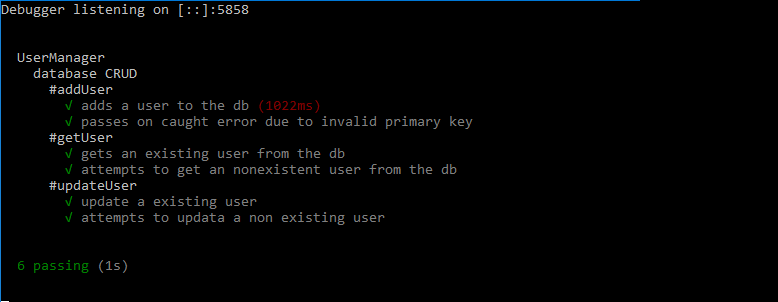
\includegraphics[width=\textwidth]{tests/usrCRUD/tests-pass.png}
		\caption{Mocha output of successful \textit{User Manager} test}
	\end{figure}
	\end{center}
	\textbf{User Manager CRUD fail example, due to Cassandra database being down. Note error reports on the console is also piped into a rotating file. Thus systems users will be able to track down errors after they occur.}
	\begin{center}
	\begin{figure}[h!]
		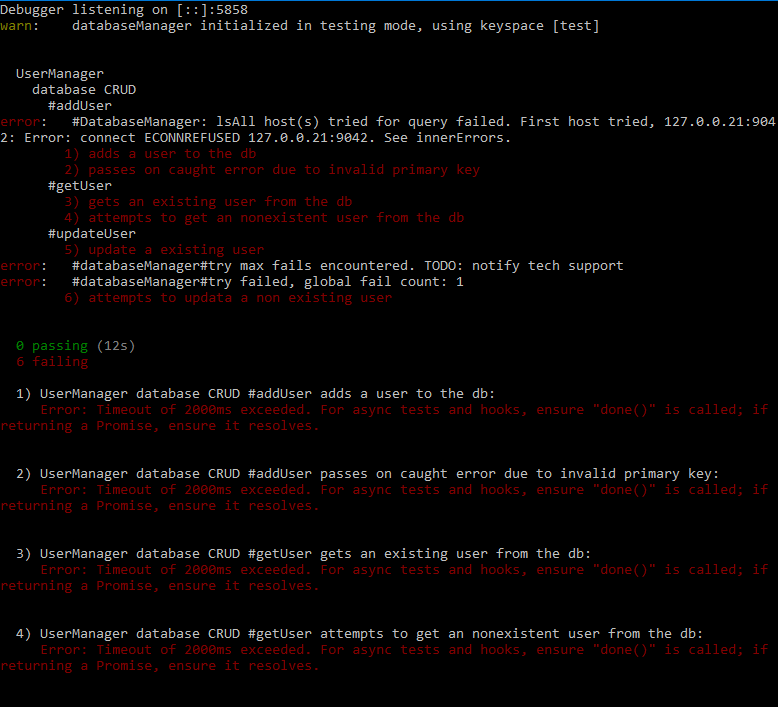
\includegraphics[width=\textwidth]{tests/usrCRUD/tests-fail.png}
		\caption{Mocha output of unsuccessful \textit{User Manager} test, due to database connection failure}
	\end{figure}
	\end{center}

%!!!!!!!!!!!!!!!!!!!!!!!!!!!!!!!!!!!!!!!!!!!!!!!!BREAK!!!!!!!!!!!!!!!!!!!!!!!!!!!!!!!!!!!!!!!!!!!!!!!
\pagebreak
%!!!!!!!!!!!!!!!!!!!!!!!!!!!!!!!!!!!!!!!!!!!!!!!!BREAK!!!!!!!!!!!!!!!!!!!!!!!!!!!!!!!!!!!!!!!!!!!!!!!

	\subsubsection{User Interface}
	\textbf{Implementation status:} partly-implemented \\
	\textbf{Primary Actors:} non-users \\
	\textbf{Functionality} Type in details and register to become a new user. There is only local validation and forms currently implemented. Client-server communication for registration and user management is not yet implemented.
	\subsubsection{Description of current tests}
	There are unit tests for each input that test the validation of those inputs. So there are tests for email, passwords, usernames etc. All to make sure that the validation is correct. \\
	\textbf{Following is the code for each unit test to show what is tested.}
	\begin{center}
	\begin{figure}[h]
		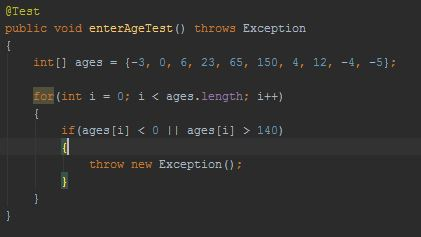
\includegraphics[width=15cm, height=5cm]{tests/usrUI/TestAge.JPG}
	\end{figure}

	\begin{figure}[h]
		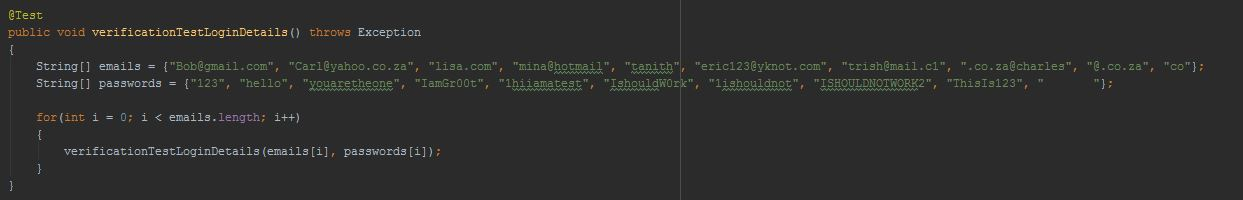
\includegraphics[width=15cm, height=4cm]{tests/usrUI/TestLogin.JPG}
	\end{figure}

	\begin{figure}[h]
		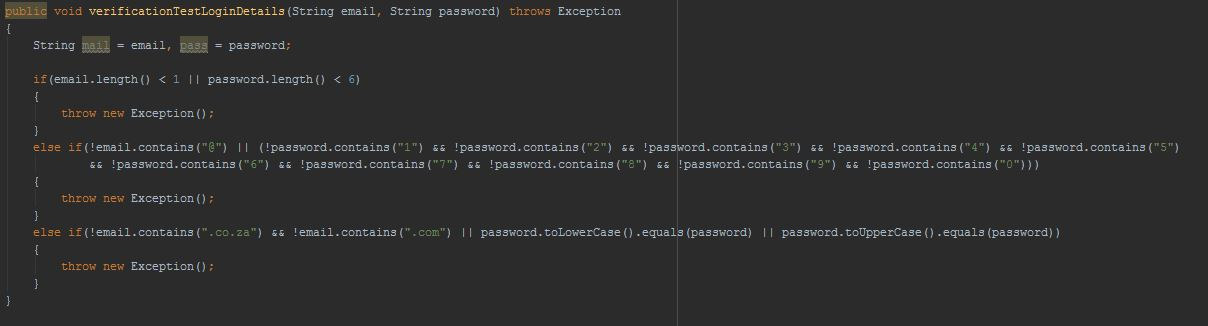
\includegraphics[width=15cm, height=7cm]{tests/usrUI/TestLoginFunction.JPG}
	\end{figure}

	\begin{figure}[h]
		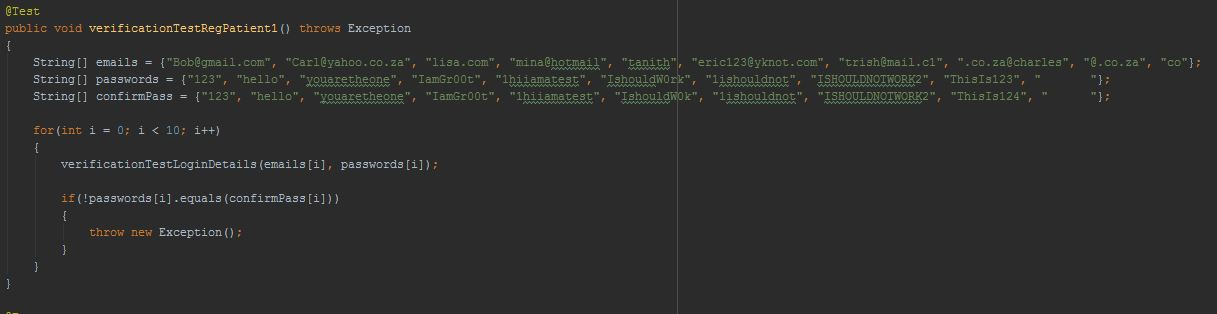
\includegraphics[width=15cm, height=5cm]{tests/usrUI/TestRegister.JPG}
	\end{figure}

	\begin{figure}[h]
		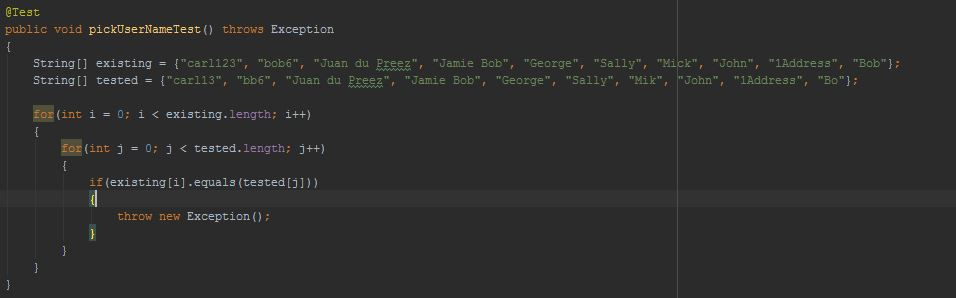
\includegraphics[width=15cm, height=4cm]{tests/usrUI/TestUsername.JPG}
	\end{figure}
	\end{center}

	\subsubsection{Future tests:}
	Integration tests that verify client-server communication is happening correctly. Functionality Tests to confirm the User Management subsystem adheres to the requirements. 

	\section{Notification Subsystem }
	\textbf{Modules involved:} Pub/Sub Server, Notification, and User Interface \\
	\textbf{Implementation status:} unimplemented \\
	\subsubsection{Future tests:}
	Unit tests for each individual module as well as integration tests to be sure messages are being passed properly between modules. 

	\section{Advice Subsystem}
	\textbf{Modules involved:} Advice and User Interface \\
	\textbf{Implementation status:} unimplemented \\
	\subsubsection{Future tests:}
	Unit tests for each individual module as well as integration tests to be sure messages are being passed properly between modules. This is made easier because both of these modules are local to the application. 

	\section{Other future tests based on non-functional requirements}
		\subsection{Usability test}
		A full usability test will be conducted with at least 6 people to determine how usable the UI on the app is. Questionairres and surveys will be used to determine where the fault lies and then improvements can be made. 
		\subsection{Accessibility test}
		Determining if the application gives affordance to people with disabilities is important, especially considering who the application is purposed for, the bedredden or very sick patients. It also allows a greater number of people to be comfortable with the app allowing more users. 

	\section{Platform compatibility test (future test)}
	Platform compatibility will be tested, so that we know devices of different screen sizes and different android versions work correctly with our application. 


\end{document}
